\chapter{Corriente alterna trifásica}
\section{Enunciado}
 
El receptor trifásico de la figura tiene secuencia de fases inversa y tensión de línea 200$\sqrt{3}$ V. Su potencia activa es 12 kW y el vatímetro 2 ($W_2$) indica 6 kW. Hallar:
\begin{itemize}
    \item Valor de la impedancia $\overline{Z}$, en forma compleja.
    \item Fasores correspondientes a las intensidades de línea.
\end{itemize}

\begin{center}
  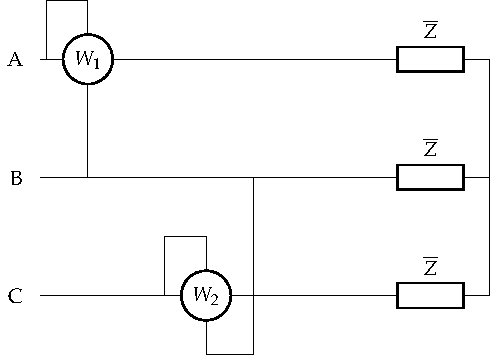
\includegraphics[width=0.45\linewidth]{figuras/ej6_BT3.pdf}
\end{center}

\subsection*{Solución}

El receptor está conectado en estrella a tres hilos (sin neutro). Al ser secuencia de fases inversa, se tiene que al principio de la línea:
\begin{align*}
    &\overline{U_{ab}}=200\sqrt{3}\phase{-120^\circ}\;\text{V} \\
    &\overline{U_{bc}}=200\sqrt{3}\phase{0^\circ}\;\text{V} \\
    &\overline{U_{ca}}=200\sqrt{3}\phase{120^\circ}\;\text{V}  \\
    &\overline{U_a}=200\phase{-90^\circ}\,V\\
    &\overline{U_b}=200\phase{30^\circ}\,V\\
    &\overline{U_c}=200\phase{150^\circ}\,V
\end{align*}

La potencia activa del receptor es 12000 W, por lo que:
\begin{equation*}
    P_T=3\cdot R_F\cdot I_F^2=3\cdot \dfrac{U_F^2}{R_F}\rightarrow R_F=3\cdot\dfrac{U_F^2}{P_T}=3\cdot \dfrac{200^2}{12000}=10\;\Omega\text{/fase}
\end{equation*}
Dado que se trata de un receptor equilibrado, por el método de los dos vatímetros, se cumple que:
\begin{equation*}
    P_T=W_1+W_2\rightarrow W_1=P_T-W_2=12000-6000=6000\;\text{W}
\end{equation*}
Con esto se puede obtener la potencia reactiva consumida por la carga. Al tratarse de una secuencia inversa:
\begin{equation*}
    Q_T=\sqrt{3}\; (W_1-W_2)=\sqrt{3}\cdot (6000-6000)=0\;\text{VAr}
\end{equation*}
Por lo que la impedancia $\overline{Z}$ es puramente resistiva de valor $\overline{Z}=10\phase{0^\circ}\Omega/fase$.

A partir de la tensión de fase, y aplicando la ley de Ohm, se puede obtener la intensidad de fase que circula por el receptor (igual a la de línea, por estar en estrella)\footnote{Con el módulo de $I_L$, podría determinarse también el valor de $\overline{Z}$ considerando la medida de $W_2$. Según el método de los dos vatímetros se sabe que $W_2=U_L\,I_L\,\cos(\theta+30)=200\sqrt{3}\cdot 20\cdot \cos(\theta+30)=6000\Rightarrow \theta = 0^\circ\Rightarrow\overline{Z}=10\Omega/fase$}:
\begin{align*}
    \overline{I_a}&=\dfrac{\overline{U_{a}}}{\overline{Z}}=\dfrac{200\phase{-90}}{10}={20\phase{-90^\circ}\;\text{A}}\\
    \overline{I_b}&=\dfrac{\overline{U_{b}}}{\overline{Z}}=\dfrac{200\phase{30}}{10}={20\phase{30^\circ}\;\text{A}}\\
    \overline{I_c}&=\dfrac{\overline{U_{c}}}{\overline{Z}}=\dfrac{200\phase{150}}{10}={20\phase{150^\circ}\;\text{A}}
\end{align*}



%%%%%%%%%%%%%%%%%%%%%%%%%%%%%%%%%%%%%%%%%%%%%%%%%%%%%%%%%%%%%%%%%%%%%%%%%

 \section{Enunciado}
 
En el sistema trifásico de la figura de secuencia de fases directa y $f=60$ Hz, el receptor equilibrado disipa una potencia total $P_T =51984$ W con un factor de potencia de 0,6 en
retraso. Sabiendo que el amperímetro indica 76$\sqrt{3}$ A,
determinar:
\begin{itemize}
    \item  Lecturas de los vatímetros 1 y 2
    \item  Valor de la impedancia $\overline{Z}$ en forma compleja
    \item Capacidad mínima para mejorar el factor de potencia a 0,95
\end{itemize}

\begin{center}
  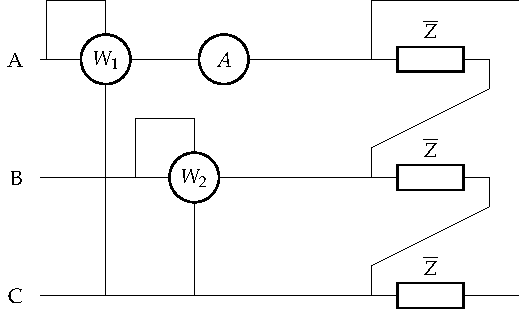
\includegraphics[width=0.4\linewidth]{figuras/ej4_BT3.pdf}
\end{center}


\subsection*{Solución}
Las tres impedancias están conectadas en triángulo. El amperímetro mide el módulo de la corriente de línea $\overline{I_a}$. Dado que se conoce el factor de potencia $\cos(\varphi)=0.6$ (en retraso), se tiene que $\varphi=+53.1301^\circ$. Por el método de los dos vatímetros:
\begin{equation*}
    P_T=W_1+W_2=51984=\sqrt{3}\, U_L\, I_L\, \cos{\phi}\rightarrow U_L=\dfrac{P_T}{\sqrt{3}\, I_L\,\cos{\phi}}=\dfrac{51984}{\sqrt{3}\cdot 76\sqrt{3}\cdot 0.6}=380\;\text{V}
\end{equation*}
por lo que: 
\begin{align*}
    W_1&=U_L\,I_L\,\cos(\phi-30^\circ)=380\cdot 76\sqrt{3}\cdot\cos(53.1301-30)=46000.65\,W\\
    W_2&=U_L\,I_L\,\cos(\phi+30^\circ)=380\cdot 76\sqrt{3}\cdot\cos(53.1301+30)=5983.35\,W
\end{align*}
  
Considerando la referencia de tensiones para SFD:
\begin{equation*}
    \overline{U_{ab}}=380\phase{120^\circ}\,V;\hfil 
    \overline{U_{bc}}=380\phase{0^\circ}\,V;\hfil 
    \overline{U_{ca}}=380\phase{-120^\circ}\,V
\end{equation*}
El módulo de las corrientes de fase es:
\begin{equation*}
    I_F=\dfrac{I_L}{\sqrt{3}}=\dfrac{76\sqrt{3}}{\sqrt{3}}=76\,A
\end{equation*}
y, dado que $\phi=\theta_U-\theta_I\rightarrow \theta_I=\theta_U-\phi$, se tiene que las corrientes de fase: 
\begin{equation*}
    \overline{I_{ab}}=76\phase{66.87^\circ}\,V;\hfil 
    \overline{I_{bc}}=76\phase{-53.13^\circ}\,V;\hfil 
    \overline{I_{ca}}=76\phase{-173.13^\circ}\,V
\end{equation*}
Por tanto, el valor de la impedancia $\overline{Z}$ es: 
\begin{equation*}
    \overline{Z}=\dfrac{\overline{U_{ab}}}{\overline{I_{ab}}}=\dfrac{\overline{U_{bc}}}{\overline{I_{bc}}}=\dfrac{\overline{U_{ca}}}{\overline{I_{ca}}}=\textbf{5\phase{53.1301^\circ}}\;\Omega={3+\mathrm{j}\,4}\;\Omega
\end{equation*}

Al indicarse que la capacidad para mejorar el factor de potencia debe ser la {mínima}, se opta por una configuración del banco de condensadores en {triángulo}. La potencia reactiva inicial $Q_T$ es:
\begin{equation*}
    Q_T=P\cdot \tan(\phi)=51984\cdot \tan(53.1301)=69312\;\text{VAr}
\end{equation*}
El nuevo factor de potencia es $\cos{\phi'}=0.95\rightarrow\phi'=18.1949^\circ$, siendo la potencia reactiva $Q_T'$:
\begin{equation*}
    Q_T'=P\cdot \tan(\phi')=51984\cdot \tan(18.1949)=17086.34\;\text{VAr}.
\end{equation*}
Por tanto, la potencia reactiva que genera la batería de condensadores a conectar es: 
\begin{equation*}
    Q_C=Q_T'-Q_T=17086.34-69312=-52225.66\;\text{VAr}
\end{equation*}
teniendo una capacidad $C$ (conectada en triángulo, $C_D$) de:
\begin{equation*}
    C_D=\dfrac{|Q_C|}{3\cdot\omega\cdot U^2}=\dfrac{52225.66}{3\cdot 2\cdot\pi\cdot 60\cdot 380^2}= \qty{319.8}{\micro\farad}
\end{equation*}



%%%%%%%%%%%%%%%%%%%%%%%%%%%%%%%%%%%%%%%%%%%%%%%%%%%%%%%%%%%%%%%%%%%%%%%%%

\section{Enunciado}
 
En el sistema trifásico de la figura, de secuencia de fases inversa y tensión de línea 200$\sqrt{3}$ V, los dos receptores son equilibrados, con impedancias $\overline{Z_1} = 6+\mathrm{j}8\;\Omega$ y $\overline{Z_2} = 8+\mathrm{j}6\;\Omega$. Determinar:
\begin{itemize}
    \item  Lecturas de los amperímetros.
    \item  Lecturas de los vatímetros y la potencia compleja total.
\end{itemize}
\begin{center}
  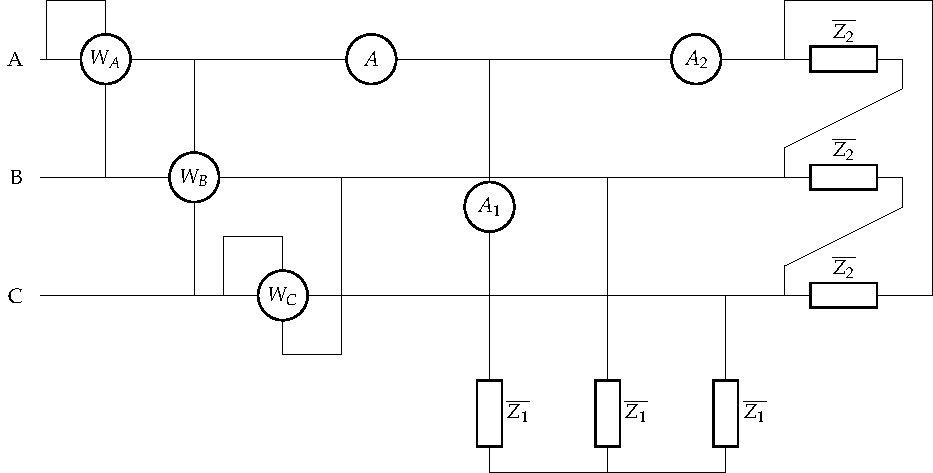
\includegraphics[width=.8\linewidth]{figuras/ej5_BT3.pdf}
\end{center}

\subsection*{Solución}
Las impedancias $\overline{Z_1}$ están conectadas en estrella, mientras que las $\overline{Z_2}$ lo están en triángulo; entre ellas, están conectadas en paralelo. 

El amperímetro $A_1$ mide la corriente de línea que va a la impedancia $\overline{Z_{1,A}}$ (módulo de $\overline{I_{1,a}}$). Puesto que se tiene la tensión de fase $\overline{U_{a}}$ y el valor de la impedancia de $\overline{Z_1}$, la corriente $\overline{I_{1,a}}$ es:
\begin{equation*}
    I_{1,a} = \frac{U_f}{Z_1} = \qty{20}{\ampere}.
\end{equation*}
por lo que el amperímetro $A_1$ marca 20 A. 

El amperímetro $A_2$ mide la corriente de línea que va a la impedancia $\overline{Z_{2,A}}$ (módulo de $\overline{I_{2,a}}$). La corriente que circula por esta impedancia (corriente de fase) es:

\begin{equation*}
    I_{2f} = \frac{U}{Z_2} = \qty[parse-numbers = false]{20\sqrt{3}}{\ampere}.
\end{equation*}

Por tanto, el amperímetro $A_2$, que marca el módulo de la corriente de línea $I_{2,a}$: 
\begin{equation*}
    I_{2,a}= \sqrt{3}\cdot I_{2f} = \qty{60}{\ampere}.
\end{equation*}
por lo que el amperímetro $A_2$ marca 60 A.

El amperímetro $A$ mide la corriente de línea $I_a$. Se puede obtener su valor mediante la LKC, para lo que sería necesario obtener los fasores de las corrientes $I_{1a}$ e $I_{2a}$ o, de forma más sencilla, mediante el Teorema de Boucherot. Las potencias de cada carga y total son:

\begin{itemize}
    \item Carga $\overline{Z_1}$:
    \begin{align*}
        P_1&=3\cdot R_1\cdot I_{F,1}^2=3\cdot 6\cdot 20^2=7200\;\text{W}\\
        Q_1&=3\cdot X_1\cdot I_{F,1}^2=3\cdot 8\cdot 20^2=9600\;\text{VAr}
    \end{align*}
    \item Carga $\overline{Z_2}$:
    \begin{align*}
        P_2&=3\cdot R_2\cdot I_{F,2}^2=3\cdot 8\cdot (20\sqrt{3})^2=28800\;\text{W}\\
        Q_2&=3\cdot X_2\cdot I_{F,2}^2=3\cdot 6\cdot (20\sqrt{3})^2=21600\;\text{VAr}
    \end{align*}
    \item Total:
    \begin{align*}
        P_T&=P_1+P_2=7200+28800=36000\;\text{W}\\
        Q_T&=Q_1+Q_2=9600+21600=31200\;\text{VAr}\\
        \overline{S_T}&=P_T+j\,Q_T={36000+\mathrm{j}\,31200 = 47638.64\phase{40.9144^\circ} \;\text{VA}}
    \end{align*}
\end{itemize}

Por tanto, teniendo en cuenta que $S_T = \sqrt{3} U \cdot I$, obtenemos la corriente de línea (lectura del amperímetro A):

\begin{equation*}
  I = \frac{47638.6}{\sqrt{3} \cdot 200\sqrt{3}} = \qty{79.4}{\ampere}.
\end{equation*}


El vatímetro $W_A$ mide la corriente de línea $A\;(I_a)$ y la tensión de línea $U_{ab}$; el vatímetro $W_B$ mide la corriente de línea $B\;(I_b)$ y la tensión de línea $U_{ac}=-U_{ca}$; por último, el vatímetro $W_C$ mide la corriente de línea $C\;(I_c)$ y la tensión de línea $U_{bc}$.

Por el método de los dos vatímetros, $W_A$ y $W_C$ miden la potencia total: 
\begin{align*}
  P_T &= W_A + W_C =\qty{36000}{\watt}\\
  Q_T &= \sqrt{3}\cdot (W_A - W_C) = \qty{31200}{\voltampere}_r
\end{align*}

Por tanto,

\begin{align*}
  W_A &= \qty{27007.43}{\watt}\\
  W_C &= \qty{8993.58}{\watt}
\end{align*}

Por otra parte, el vatímetro $W_B$ mide la potencia reactiva total entre $\sqrt{3}$:
\begin{equation*}
  W_B = Q_T/\sqrt{3}=\qty{18013.85}{\watt}
\end{equation*}


%%%%%%%%%%%%%%%%%%%%%%%%%%%%%%%%%%%%%%%%%%%%%%%%%%%%%%%%%%%%%%%%%%%%%%%%%

\section{Enunciado}
 
El sistema trifásico de la figura es de 380 V a 50 Hz y secuencia de fases inversa. $\overline{Z}$ es un elemento pasivo ideal, tal que el factor global de potencia es la unidad. El motor es de 1,8 CV, rendimiento 90\% y factor de potencia 0,8. Determinar:
\begin{itemize}
    \item  Impedancia $\overline{Z}$ en forma compleja.
    \item  Intensidad en el motor.
    \item  Fasores intensidad de línea.
    \item  Lectura de los aparatos de medida: V, A, W$_1$, W$_2$ y W$_3$.
\end{itemize}
\begin{center}
  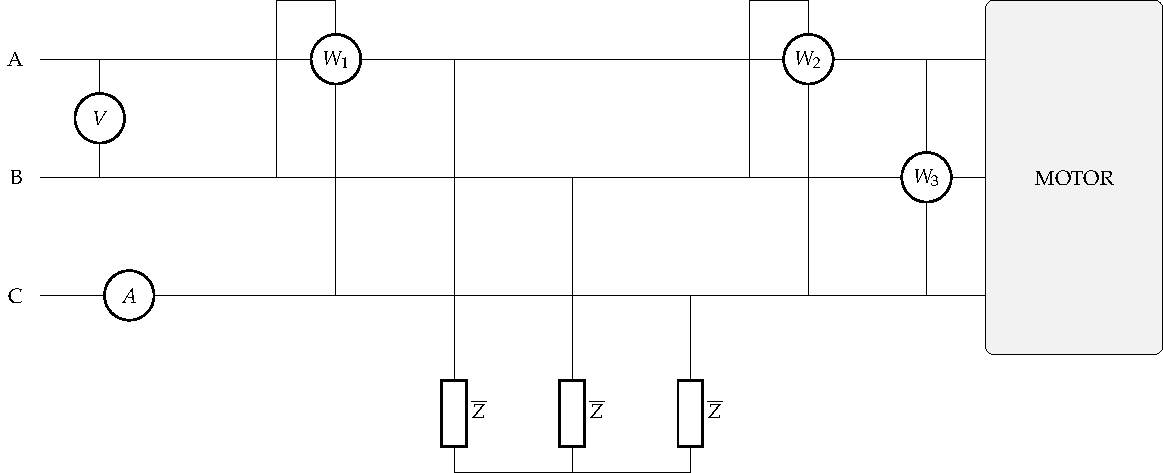
\includegraphics[width=\linewidth]{figuras/ej7_BT3.pdf}
\end{center}

\subsection*{Solución}
El motor tiene una potencia útil de 1.8 CV que, en W:
\begin{equation*}
  P_u=1.8\cdot 746=1342.8\;\text{W}    
\end{equation*}
Su potencia activa, considerando el rendimiento, es:
\begin{equation*}
  P_M=\dfrac{P_u}{\eta}=\dfrac{1342.8}{0.9}=1492\;\text{W}
\end{equation*} 


Al ser secuencia de fases inversa, se tiene que al principio de la
línea:
\begin{align*}
  &\overline{U_{ab}}=380\phase{-120^\circ}\;\text{V} \\
  &\overline{U_{bc}}=380\phase{0^\circ}\;\text{V} \\
  &\overline{U_{ca}}=380\phase{120^\circ}\;\text{V}  \\
  &\overline{U_a}=220\phase{-90^\circ}\,V\\
  &\overline{U_b}=220\phase{30^\circ}\,V\\
  &\overline{U_c}=220\phase{150^\circ}\,V
\end{align*}

Se sabe que el factor de potencia global es 1. Dado que el motor tiene
un comportamiento inductivo, con factor de potencia de $0.8$, y la
impedancia $\overline{Z}$ es un elemento pasivo ideal, {ésta debe ser
  una batería de condensadores} conectados en estrella que mejoren el
factor de potencia a 1. La potencia reactiva del motor $Q_M$ es:
\begin{equation*}
  Q_M=P_M\cdot \tan(\phi_M)=1492\cdot \tan(36.8699)=1119\;\text{VAr}
\end{equation*}
El factor de potencia global es $\cos{\phi}=1\rightarrow\phi=0^\circ$,
siendo la potencia reactiva $Q_T$:
\begin{equation*}
  Q_T=P_M\cdot \tan(\phi)=1492\cdot \tan(0)=0\;\text{VAr}
\end{equation*}
Por tanto, la potencia reactiva que genera la batería de condensadores
(impedancia $\overline{Z}$) es:
\begin{equation*}
  Q_Z=Q_T-Q_M=0-1119=-1119\;\text{VAr}
\end{equation*}
que, al estar conectados en estrella, tienen una impedancia de:
\begin{equation*}
  Q_Z=3\cdot \dfrac{U_F^2}{Z}\rightarrow Z=3\cdot \dfrac{U_F^2}{Q_Z}=3\cdot \dfrac{220^2}{-1119}=-129.76\;\Omega\rightarrow \overline{Z}={-\mathrm{j}\,129.76}\;\Omega\text{/fase}
\end{equation*}

La intensidad en el motor es:
\begin{equation*}
  I_M=\dfrac{P_M}{\sqrt{3}\,U_L\,\cos(\phi_M)}=\dfrac{1492}{\sqrt{3}\cdot 380\cdot 0.8}=2.83\,A
\end{equation*}

Dado que los condensadores no consumen potencia activa, las
intensidades de línea se pueden calcular a partir de la potencia
activa consumida por el motor, y el factor de potencia global de la
instalación:
\begin{equation*}
  I_L=\dfrac{P_T}{\sqrt{3}\cdot U_L\cdot \cos{(\phi})}=\dfrac{1492}{\sqrt{3}\cdot 380\cdot 1}=2.27\;\text{A}
\end{equation*}
que, en forma fasorial, teniendo en cuenta que $\phi'=0^\circ$:
\begin{align*}
  \overline{I_{a}}&={2.27\phase{-90^\circ}\;\text{A}}\\
  \overline{I_{b}}&={2.27\phase{30^\circ}\;\text{A}}\\
  \overline{I_{c}}&={2.27\phase{150^\circ}\;\text{A}}
\end{align*}

El voltímetro $V$ mide el módulo de la tensión
$\overline{U_{ab}}\rightarrow V={380}$ {V}. El amperímetro $A$ mide el
módulo de la corriente $\overline{I_c}\rightarrow A={2.27}$ {A}. El
vatímetro $W_1$ mide la corriente $\overline{I_a}$ y la tensión
$\overline{U_{bc}}$, por lo que:
\begin{equation*}
  W_1=U_{bc}\cdot I_a\cdot \cos{(\theta_{{U}_{bc}}-\theta_{{I}_a})}= 380\cdot 2.27\cdot \cos(0-(-90))={0\;\text{W}}
\end{equation*}

También podemos obtener este valor teniendo en cuenta que, por la
conexión que tiene, y al tratarse de SFI, está midiendo
$-Q_T/\sqrt{3}$. Al tener la instalación en su conjunto un
$\cos(\phi)=0$, la potencia reactiva total es $Q_T=0$, por lo que
$W_1=0$ W.
  
El vatímetro $W_2$ mide la corriente $\overline{I_{a,M}}$ y la tensión
$\overline{U_{bc}}$. El ángulo de $\overline{I_{a,M}}$, considerando
que el motor está conectado en estrella, es
$\theta_{I_{a,M}}=\theta_{U_{a,M}}-\phi_M=-90-(-36.8699)=126.8699^\circ$,
por lo que:
\begin{equation*}
  W_2=U_{bc}\cdot I_{a,M}\cdot \cos{(\theta_{{U}_{bc}}-\theta_{{I}_{a,M}})}= 380\cdot 2.83\cdot \cos(0-126.8699)={-645.24\;\text{W}}
\end{equation*}
Como alternativa, viendo la conexión que tiene, y al tratarse de SFI,
se sabe que está midiendo $-Q_M/\sqrt{3}$. Al tener el motor una
$Q_M=1119$ VAr, $W_2=-1119/\sqrt{3}=-646.05$ W.
  
Por último, el vatímetro $W_3$ mide el módulo de la corriente
$\overline{I_{b,M}}$ y de la tensión $\overline{U_{ac}}$. El ángulo de
$\overline{I_{b,M}}$, considerando que el motor está conectado en
estrella, es
$\theta_{I_{b,M}}=\theta_{U_{b,M}}-\phi_M=30-(-36.8699)=66.8699^\circ$;
y el ángulo de
$\overline{U_{ac}}=-\overline{U_{ca}}=380\phase{-60^\circ}$, por lo
que:
\begin{equation*}
  W_3=U_{ac}\cdot I_{b,M}\cdot \cos{(\theta_{{U}_{ac}}-\theta_{{I}_{b,M}})}= 380\cdot 2.83\cdot \cos(-60-66.8699)={645.24\;\text{W;}}
\end{equation*}

De otra forma, por la conexión que tiene, y al tratarse de SFI, se
sabe que está midiendo $Q_M/\sqrt{3}$, por lo que
$W_3=1119/\sqrt{3}=646.05$ W.


 \section{Enunciado}

 Una plantación agrícola emplea dos bombas sumergibles para extraer
 agua de un pozo y transportarla a través de un sistema de riego por
 goteo. Estas dos bombas están alimentadas a \SI{400}{\volt} por una
 línea trifásica en secuencia de fases directa y frecuencia
 $\SI{50}{\hertz}$. Una de las bombas funciona con un motor trifásico
 de $\SI{30}{\kilo\watt}$ y factor de potencia de 0.78. La otra bomba
 trabaja con un motor de $\SI{7.5}{\kilo\watt}$ y factor de potencia
 de 0.67.  La línea que alimenta estas dos bombas es resistiva, con
 resistividad $\rho = \SI{0.017}{\ohm\milli\meter\squared\per\meter}$,
 longitud de \SI{300}{m} y una sección de
 \SI{35}{\milli\meter\squared}.
 
 \begin{enumerate}
 \item Calcula el triángulo de potencias (potencia activa, reactiva, y
   aparente) de cada carga, y total de las cargas (a la salida de la
   línea).
 \item Calcula el \textbf{valor eficaz} de la corriente de línea de
   cada carga, y total.
 \item Determine la lectura de los siguientes aparatos de medida
   conectados a la entrada de las cargas:
   \begin{itemize}
   \item Un vatímetro en la fase A, midiendo tensión entre las fases A
     y C.
   \item Un vatímetro en la fase B, midiendo tensión entre las fases B
     y C.
   \item Un vatímetro en la fase C, midiendo tensión entre las fases B
     y A.
   \end{itemize}
 \item Calcule el triángulo de potencias a la entrada de la línea.
 \item Calcule el \textbf{valor eficaz} de la tensión a la entrada de la línea.
 \item Calcule los condensadores que se deben conectar a la salida de
   la línea para mejorar el factor de potencia del sistema hasta la
   unidad. Indique el modo de conexión.
 \end{enumerate}

Una vez conectados los condensadores del último apartado:
\begin{enumerate}[resume]
\item Calcule el \textbf{valor eficaz} de la corriente de línea total.
\item Calcule el triángulo de potencias a la entrada de la línea.
\item Calcule el \textbf{valor eficaz} de la tensión a la entrada de la línea.
\item Determine la lectura de los vatímetros descritos anteriormente.
\end{enumerate}

\subsection*{Solución}

 Las potencias de cada carga son:
 \begin{align*}
   P_1 &= \SI{30}{\kilo\watt}\\
   Q_1 &= P_1\tan \theta_1 = \SI{24.06}{\kilo\voltampere}_r\\
   S_1 &= \SI{38.46}{\kilo\voltampere}\\
   P_2 &= \SI{7.5}{\kilo\watt}\\
   Q_2 &= P_2 \tan \theta_2 = \SI{8.31}{\kilo\voltampere}_r\\
   S_2 &= \SI{11.19}{\kilo\voltampere}
 \end{align*}

 Aplicando Boucherot, el triángulo de potencias total es:
 \begin{align*}
   P_T &= \SI{37.5}{\kilo\watt}\\
   Q_T &= \SI{32.37}{\kilo\voltampere}_r\\
   S_T &= \sqrt{P_T^2 + Q_T^2} = \SI{49.54}{\kilo\voltampere}
 \end{align*}

 Por tanto, el ángulo de la impedancia global es:

\[
  \tan(\theta) = \frac{Q_T}{P_T} = 0.8632 \rightarrow \theta =
  \ang{40.8}
\]

Las corrientes en cada carga son:

\begin{align*}
  I_1 &= \frac{S_1}{\sqrt{3} U} = \SI{55.51}{\ampere}\\
  I_2 &= \frac{S_2}{\sqrt{3} U} = \SI{16.15}{\ampere}
\end{align*}

La corriente total es:
\[
  I = S_T /{\sqrt{3} U} = \SI{71.5}{\ampere}
\]

Denominaremos con $W_1$ al vatímetro conectado en la fase A midiendo
tensión entre las fases A y C, y con $W_2$ al vatímetro conectado en
la fase B midiendo tensión entre las fases B y C. Teniendo en cuenta
que se trata de una SFD:
 
\begin{align*}
  W_1 + W_2 &= P_T\\
  W_1 - W_2 &= Q_T/\sqrt{3}
\end{align*}

Por tanto:

\begin{align*}
  W_1 &= 1/2 (P_T + Q_T/\sqrt{3}) = \SI{28.09}{\kilo\watt}\\
  W_2 &= 1/2 (P_T - Q_T/\sqrt{3}) = \SI{9.41}{\kilo\watt}
\end{align*}

También podemos obtener estos resultados con las siguientes
ecuaciones:

\begin{align*}
  W_1 &= U I \cos(\theta - \ang{30}) = \SI{28.09}{\kilo\watt}\\
  W_2 &= U I \cos(\theta + \ang{30}) = \SI{9.41}{\kilo\watt}
\end{align*}

Por otra parte, el vatímetro de la fase C mide:

\[
  W_{C, BA} = - \frac{Q_T}{\sqrt{3}} = - \SI{18.66}{\kilo\watt}
\]

La resistencia de la línea (una resistencia por cada conductor) es:

\[
R_L = \rho L/S = \SI{0.146}{\ohm}
\]

La potencia activa disipada en la línea es:

\[
P_L = 3 \cdot I^2 R_L = \SI{2234.8}{\watt}
\]

Por tanto, la potencia a la entrada de la línea es:

\begin{align*}
P_g &= P_L + P_T = \SI{39.73}{\kilo\watt}\\
Q_g &= Q_T = \SI{32.33}{\kilo\voltampere}_r\\
S_g &= \SI{51.22}{\kilo\voltampere}
\end{align*}

Y la tensión a la salida del generador (entrada de la línea) es:

\[
U_g = \frac{S_g}{\sqrt{3} I} = \SI{413.64}{\volt}
\]

Para mejorar el factor de potencia a la unidad en las cargas, se necesita una batería de condensadores conectados en triángulo en las cargas (a la salida de la línea). Cada uno de los tres condensadores debe tener una capacidad de:

\[
C = \frac{Q_T}{3 \omega U^2} = \SI{214.4}{\micro\farad}
\]

Una vez instalada la batería de condensadores, la corriente total a la salida de la línea es:

\[
I' = \frac{P_T}{\sqrt{3} U} = \SI{54.13}{\ampere}
\]

La potencia disipada en la línea es ahora:

\[
P'_L = 3 \cdot I'^2 R_L = \SI{1282.9}{\watt} 
\]

Por tanto, el triángulo de potencias a la entrada de la línea es:
\begin{align*}
P'_g &= \SI{38.78}{\kilo\watt}\\
Q'_g &= \SI{0}{\kilo\voltampere}_r\\
S'_g &= \SI{38.78}{\kilo\voltampere}
\end{align*}

Consecuentemente, la tensión a la entrada de la línea es:

\[
U' = \frac{S'_g}{\sqrt{3} I'} = \SI{413.63}{\volt}
\]

Con la inserción de los condensadores los vatímetros miden:

\begin{align*}
W'_{A, AC} = W'_{B, BC} &= 1/2 \cdot P'_T = \SI{18.75}{\kilo\watt}\\
W'_{C, BA} &= \SI{0}{\watt}
\end{align*}



\section{Enunciado}

El circuito de la figura es de secuencia de fases directa y 50 Hz. Determinar:
\begin{enumerate}
\item Potencias activas y reactivas totales.
\item Capacidad mínima de los condensadores a instalar para mejorar el factor de potencia total hasta la unidad.
\item Intensidades de línea, en forma fasorial, una vez mejorado el factor de potencia.
\end{enumerate}
\begin{minipage}{0.4\linewidth}
  Datos: 

  \begin{align*}
    \overline{Z}_1 &= {100\phase{\ang{60}}}\unit{\ohm}\\
    W_1 &= \SI{300}{\watt}\\
    W_2 &= \SI{300}{\watt}\\
    V &= {\sqrt{3} \cdot 200}\unit{\volt}
  \end{align*}
\end{minipage}
\begin{minipage}{0.6\linewidth}
  \begin{center}
    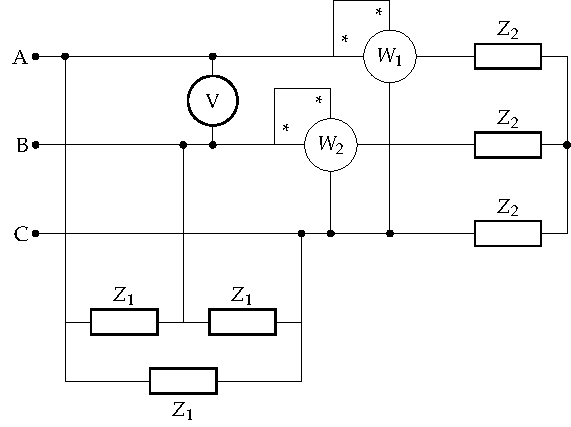
\includegraphics{figuras/ZyZt}
  \end{center}
\end{minipage}

\subsection*{Solución}

Los dos vatímetros miden la potencia de la impedancia $Z_2$:

\begin{align*}
  P_2 &= W_1 + W_2 = \SI{600}{\watt}\\
  Q_2 &= \sqrt{3}\cdot (W_1 - W_2) = \SI{0}{\volt\ampere_r}
\end{align*}

Para calcular la potencia de $Z_2$ debemos obtener la corriente de fase:

\[
  I_{1f} = \frac{U}{Z_1} = {2\sqrt{3}}\unit{\ampere}
\]

Por tanto,

\begin{align*}
  P_1 &= 3 \cdot I_{1f}^2 R_1 = 3 \cdot (2\sqrt{3})^2 \cdot (100\cos(\ang{60})) = \SI{1800}{\watt}\\
  Q_1 &= 3 \cdot I_{1f}^2 X_1 = 3 \cdot (2\sqrt{3})^2 \cdot (100\sin(\ang{60})) = {1800\sqrt{3}}\unit{\volt\ampere_r}
\end{align*}

Aplicando Boucherot:

\begin{align*}
  P &= P_1 + P_2 = \SI{2400}{\watt}\\
  Q &= Q_1 + Q_2 = {1800\sqrt{3}}\unit{\volt\ampere_r}
\end{align*}

Se deben instalar tres condensadores en triángulo con capacidad:

\[
  C_\triangle = \frac{Q}{3 \cdot \omega U^2} = \SI{27.57}{\micro\farad}
\]

Al instalar estos condensadores la corriente que circula por la línea es:

\[
  P = \sqrt{3} \cdot U \cdot I' \rightarrow I' = \SI{4}{\ampere}
\]

En forma fasorial, teniendo en cuenta que $\theta' = \ang{0}$:

\begin{align*}
  \overline{I}_A &= {4\phase{\ang{90}}}\unit{\ampere}\\
  \overline{I}_B &= {4\phase{\ang{-30}}}\unit{\ampere}\\
  \overline{I}_C &= {4\phase{\ang{-150}}}\unit{\ampere}
\end{align*}





\section{Enunciado}

En la figura dos vatímetros miden una carga trifásica inductiva
equilibrada alimentada a una tensión $U = \SI{400}{\volt}$. El
vatímetro $W_B$ indica una lectura de \SI{11320}{\watt}, y el
vatímetro $W_C$ indica una lectura de \SI{1815}{\watt}. A partir de
esta información se pide:

\begin{enumerate}
\item Determinar la secuencia de fases del sistema.
\item Triángulo de potencias de la carga.
\item Impedancia equivalente de la carga en estrella y
  en triángulo.
\item Tensión de alimentación a la entrada de la línea
  $U_1$ sabiendo que la línea de alimentación es resistiva pura con
  valor $R = \SI{0.1}{\ohm}$.
\item Capacidad de los condensadores que se deben
  conectar en bornes de la carga para conseguir mejorar su factor de
  potencia a la unidad. Determinar las nuevas lecturas de los
  vatímetros $W_B$ y $W_c$.
\end{enumerate}

\begin{center}
  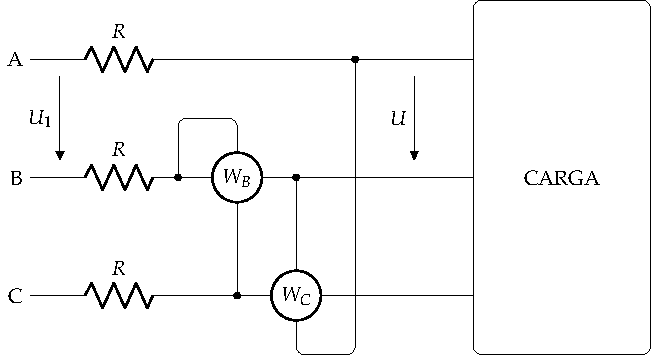
\includegraphics[width=0.6\linewidth]{figuras/BT3_10.pdf}
\end{center}

\subsection*{Solución}

El vatímetro $W_c$ está conectado de forma que mide la potencia
reactiva:

\[
  W_c = \pm \frac{Q}{\sqrt{3}}
\]

Dado que el vatímetro está conectado entre B y A, el signo negativo
corresponde a SFD y el positivo a SFI. Dado que la carga es inductiva
es $Q > 0$. Como $W_c > 0$ debemos elegir el signo positivo, lo que
implica SFI.

Al vatímetro $W_B$ podríamos añadirle un hipotético vatímetro
$W_A$ conectado en la fase A midiendo tensión entre A y C para
emplear el método de los dos vatímetros:


\begin{align*}
W_B + W_A &= P\\
W_B - W_A &= \frac{Q}{\sqrt{3}} = W_c
\end{align*}

Sumando ambas ecuaciones obtenemos:

\[
  P = 2 W_B - W_c = \SI{20825}{\watt}
\]

La potencia reactiva se calcula directamente con el vatímetro $W_c$:

\[
  Q = \sqrt{3} W_c = \SI{3143.7}{VA}_r
\]

Por tanto:

\[
  \overline{S} =
  21060.9\phase{\ang{8.58}}\unit{VA}
\]

El módulo de la impedancia en triángulo se obtiene con
$Z_{\triangle} = U / I_f$. Teniendo en cuenta que $S = \sqrt{3} U I$
y que $I = \sqrt{3} I_f$, obtenemos $I_f = S / 3U$. Por tanto
\[
  \overline{Z}_{\triangle} = \frac{3 U^2}{S}\phase{\ang{8.58}} =
  {22.8\phase{\ang{8.58}}}\unit{\ohm}
\]


Para obtener la impedancia en estrella basta con usar las relaciones
entre tensiones y corrientes de fase y línea:

\begin{align*}
  Z_Y &= \frac{U_f}{I} = \frac{1}{\sqrt{3}} \cdot \frac{U}{I}\\
  Z_\triangle &= \frac{U}{I_f} = \sqrt{3} \cdot \frac{U}{I}
\end{align*}

Por tanto, $\overline{Z}_{Y} = \overline{Z}_{\triangle} / 3$.

La corriente de línea es:

\[
  I = \frac{S}{\sqrt{3} U} = \SI{30.4}{\ampere}
\]

La potencia disipada en la línea es:

\[
  P_L = 3 \cdot I^2 \cdot R_L = \SI{277.23}{\watt}
\]

La potencia aparente total a la entrada de la línea es:

\[
  S_T = \sqrt{(P + P_L)^2 + Q^2} = \SI{21335.1}{VA}
\]

Y, por tanto,

\[
  U_1 = \frac{S_T}{\sqrt{3} I} = \SI{405.21}{\volt}
\]

Suponiendo $f = \SI{50}{\hertz}$:
\[
  C = \frac{Q}{3 \omega U^2} = \SI{20.85}{\micro\farad}
\]

Ahora, dado que $Q' = \SI{0}{VA}_r$, será $W_C = \SI{0}{\watt}$ y
$W_B = P/2 = \SI{10412.5}{\watt}$.



\section{Enunciado}

Del circuito de la figura se sabe que tiene una secuencia de fases
directa ABC. El amperímetro indica $\SI{5}{\ampere}$, el voltímetro
$\SI{400}{\volt}$, y los vatímetros A y C muestran una lectura
idéntica. Se pide:

\begin{enumerate}
\item Valor de la impedancia Z en forma compleja.
\item Expresión fasorial de todas las intensidades del circuito.
\item Lecturas de los vatímetros A y C.
\end{enumerate}

\begin{center}
  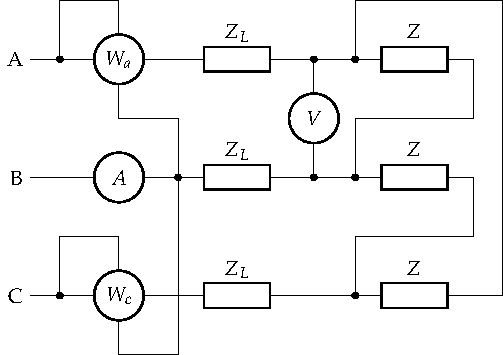
\includegraphics[width = 0.6\textwidth]{figuras/BT3_12}
\end{center}

Dato: $\overline{Z}_L = \SI[parse-numbers = false]{1 + j}{\ohm}$.

\subsection*{Solución}

Al ser un circuito equilibrado, las intensidades de fase, que
circulan por las impedancias del triángulo, tienen un valor de
$\SI[parse-numbers=false]{5/\sqrt{3}}{\volt}$. La impedancia Z
tendrá un módulo de valor:

\[
  Z = \frac{400}{5\sqrt{3}/3} =
  \SI[parse-numbers=false]{80\sqrt{3}}{\ohm}
\]

Como los vatímetros $W_a$ y $W_c$ indican el mismo valor, el
circuito tiene característica resistiva pura y por tanto, la
potencia reactiva consumida por la reactancia inductiva de las
líneas será igual pero de tipo contrario que la potencia reactiva
aportada por la reactancia capacitiva de la impedancia Z. Por tanto:

\begin{align*}
  Q_{linea} = 3 \cdot 5^2 \cdot 1 &= \SI{75}{\volt\ampere}_r\\
  Q_Z &= -\SI{75}{\volt\ampere}_r\\
  X_Z &= \SI{3}{\ohm}
\end{align*}

Por tanto:

\[
  R_Z = \sqrt{Z^2 - X_c^2} = \SI{138.5}{\ohm} \rightarrow \overline{Z} = \SI[parse-numbers=false]{138.5 - j3}{\ohm}
\]

Tomando como referencia las tensiones de secuencia directa ABC
\textbf{en el triángulo de impedancias Z}, se obtienen las siguientes
intensidades de fase:

\begin{align*}
  I_{ab} &= {2.88\phase{121.24^\circ}}\unit{\ampere}\\
  I_{bc} &= {2.88\phase{1.24^\circ}}\unit{\ampere}\\
  I_{ca} &= {2.88\phase{-118.75^\circ}}\unit{\ampere}\\
\end{align*}

A partir de estas corrientes de fase, se obtienen las corrientes de línea.
\begin{align*}
  I_{a} &= {5\phase{91.24^\circ}}\unit{\ampere}\\
  I_{b} &= {5\phase{-28.75^\circ}}\unit{\ampere}\\
  I_{c} &= {5\phase{-148.75^\circ}}\unit{\ampere}
\end{align*}



Dado que ambos vatímetros marcan el mismo valor, el circuito es
resistivo. Este valor se corresponde con la mitad de la potencia
activa total consumida por el circuito. Calculamos esta potencia con Boucherot:


\begin{align*}
  P_{ZL} &= 3 \cdot 5^2 \cdot 1\\
  P_Z &= 3 \cdot 2.88^2 \cdot 138.53\\
  P &= P_{ZL} + P_{Z} = \SI{3522.07}{\watt}
\end{align*}

\[
  W_a = W_c = 1/2 \cdot P = \SI{1761.04}{\watt}
\]



\section{Enunciado}

En el circuito de la figura se debe determinar:

\begin{center}
  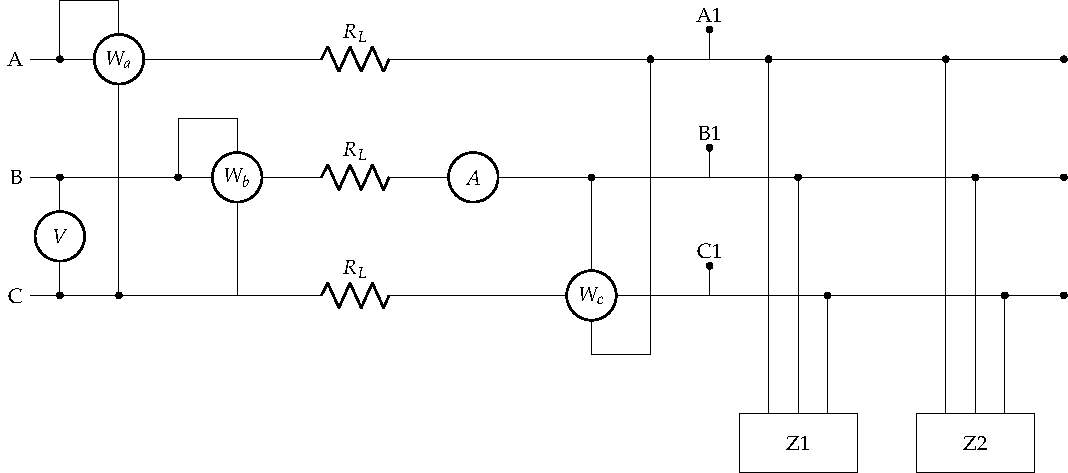
\includegraphics[width=0.9\textwidth]{figuras/BT3_11.pdf}
\end{center}

\begin{enumerate}
\item Lectura del vatímetro $W_c$.
\item Lectura del amperímetro.
\item Factor de potencia total de las cargas (en retraso o
  adelanto).
\item Lectura de los vatímetros $W_a$ y $W_b$.
\item Lectura del voltímetro.
\item Valor de los condensadores conectados en $A_1B_1C_1$ para
  que el f.d.p. en ese punto sea la unidad.
\item Lecturas de los cinco aparatos de medida tras el apartado
  anterior.
\end{enumerate}

Datos:
\begin{itemize}
\item Secuencia de fases directa, $f = \SI{50}{\hertz}$, ($A_1B_1C_1$)
  $U_1 = \SI{420}{\volt}$.
\item $Z_1$: motor de 10 CV, con $\eta = 0.83$, y f.d.p. de 0'9.
\item $Z_2$: conjunto de iluminación fluorescente, con
  $P = \SI{2400}{\watt}$, y f.d.p. de 0'85.
\item $R_L = \SI{1}{\ohm}$.
\end{itemize}

\subsection*{Solución}

A partir de los datos del enunciado, teniendo en cuenta que las dos
cargas son inductivas, obtenemos:
\begin{align*}
  P_1 &= \SI{8867.5}{\watt}\\
  Q_1 &= \SI{4294.7}{VA}_r\\
  P_2 &= \SI{2400}{\watt}\\
  Q_2 &= \SI{1487.4}{VA}_r\\
\end{align*}
Por tanto, el triángulo de potencias de las cargas ($A_1B_1C_1$) es:
\begin{align*}
  P &= \SI{11267.5}{\watt}\\
  Q &= \SI{5782.1}{VA}_r\\
  S &= \SI{12664.5}{VA}\\
\end{align*}

Dado que se trata de un sistema de SFD, la lectura del vatímetro $W_c$
es:

\begin{equation*}
  W_c = - \frac{Q}{\sqrt{3}} = \SI{-3338.3}{\watt}
\end{equation*}

La lectura del amperímetro es:

\begin{equation*}
  A = \frac{S}{\sqrt{3} U} = \SI{17.41}{\ampere}
\end{equation*}

El factor de potencia de las cargas es:

\begin{equation*}
  fdp = \cos{\arctan{\frac{Q}{P}}} = 0.89
\end{equation*}

La potencia disipada en la línea es:

\begin{equation*}
  P_L = 3 \cdot I^2 \cdot R_L = \SI{909.32}{\watt}
\end{equation*}

Y, por tanto, el triángulo de potencias total es:

\begin{align*}
  P_T = P + P_L &= \SI{12176.8}{\watt}\\
  Q_T = Q &= \SI{5782.1}{VA}_r\\
  S_T &= \SI{13479.9}{VA}
\end{align*}

Teniendo en cuenta que:

\begin{align*}
  W_A + W_B &= P_T\\
  W_A - W_B &= Q_T / \sqrt{3}
\end{align*}

obtenemos

\begin{align*}
  W_A &= \SI{7757.6}{\watt}\\
  W_B &= \SI{4419.27}{\watt}
\end{align*}

La tensión a la entrada de la línea es:

\begin{equation*}
  U' = \frac{S_T}{\sqrt{3} I} = \SI{447.02}{\volt}
\end{equation*}

Los condensadores necesarios (conectados en triángulo) deben tener una
capacidad de:

\begin{equation*}
  C = \frac{Q_T}{3U^2\omega} = \SI{34.78}{\micro\farad}
\end{equation*}

Con estos condensadores conectados, las lecturas de los aparatos de
medida son:

\begin{align*}
  W_c &= 0\\
  A &= \SI{15.5}{\ampere}\\
  P_L &= \SI{720.75}{\watt}\\
  P_T &= \SI{11988.25}{\watt}\\
  W_A = W_B &= \SI{5994.1}{\watt}\\
  U' &= \SI{446.5}{\volt}\\  
\end{align*}



\section{Enunciado}

Una línea ideal trifásica de 4 hilos alimenta a dos cargas a una
tensión de $\SI{400}{\volt}$ en secuencia de fases inversa (SFI) y
frecuencia $\SI{50}{\hertz}$.

Las cargas tienen las siguientes características:

\begin{itemize}
\item Un motor trifásico de $\SI{70}{\kilo\watt}$ y f.d.p. de 0.8.
\item Un conjunto equilibrado de 90 lámparas fluorescentes. Las
  características de cada lámpara son: potencia de $\SI{12}{\watt}$,
  f.d.p. de 0.7 en retraso, tensión $\SI{230}{\volt}$.
\end{itemize}

Con esta información se pide:

\begin{enumerate}
\item Conectar adecuadamente los siguientes aparatos de medida antes
  de las cargas.
  \begin{itemize}
  \item Un voltímetro que mida la tensión de línea (etiquetado como
    $V_L$) y otro voltímetro que mida la tensión de fase (etiquetado
    como $V_F$).
  \item Un vatímetro que permita calcular la potencia reactiva total
    del sistema (etiquetado como $W_r$).
  \item Dos vatímetros que, de forma conjunta, permitan calcular la
    potencia activa total del sistema (etiquetados como $W_X$ y
    $W_Y$).
  \end{itemize}
\item Calcular el valor eficaz de la corriente de línea
  total.
\item Calcular la lectura de cada uno de los aparatos
  de medida del primer apartado.
\item Calcular los condensadores necesarios para
  mejorar el factor de potencia hasta 0,9, indicando cómo se deben
  conectar.
\item Una vez conectados los condensadores del anterior
  apartado, determinar la corriente de línea y la lectura de todos los
  aparatos de medida del apartado 2.
\end{enumerate}

\subsection*{Solución}

El motor consume una potencia activa de $P_m = 70\mathrm{kW}$. Su
potencia reactiva es
$Q_m = P_m \cdot \tan(\theta_m) = 52.5\mathrm{kVAr}$.  Las lámparas
consumen una potencia activa de $P_f = 90 \cdot 12 =
1080\mathrm{W}$. Su potencia reactiva (inductiva) es
$Q_f = 1101.8\mathrm{VAr}$.  Aplicando Boucherot, la potencia activa
total es $P = P_m + P_f = 71.08\mathrm{kW}$ y la potencia reactiva
total es $Q = Q_m + Q_f = 53.6\mathrm{kVAr}$. Con estas magnitudes
podemos calcular el factor de potencia global, $\cos(\theta) =
0.798$. Finalmente, la corriente de línea es:

\[
  I = \frac{P}{\sqrt(3) \cdot U \cdot \cos(\theta)} = 128.5\mathrm{A}
\]


Teniendo en cuenta que es un sistema equilibrado y que es SFI,

\begin{itemize}

\item Para medir la tensión de línea hay que conectar un voltímetro
  entre dos fases. La medida será $V_{L} = 400\mathrm{V}$. Para medir
  la tensión de fase hay que conectar un voltímetro entre una fase y
  el neutro.$V_{AN} = 400 / \sqrt{3} = 230.9\mathrm{V}$

\item Hay que conectar un vatímetro midiendo tensión entre dos fases y
  la corriente por la tercera. Para que la medida coincida en signo
  con la de la potencia reactiva, la conexión entre fases debe ser BA,
  CB, o AC. Así, por ejemplo, un vatímetro midiendo tensión entre A y
  C, y corriente por B medirá $W_R = Q / \sqrt{3} = 30947\mathrm{W}$

\item Hay que usar el método de Aron. Una posibilidad es conectar un
  vatímetro midiendo tensión entre las fases A y C, y corriente en A
  ($W_X$), y otro vatímetro midiendo tensión entre las fases B y C, y
  corriente por B ($W_Y$). Para obtener la potencia activa total del
  sistema basta con sumar las dos medidas: $W_{X} + W_{Y} =
  P$. Además, podemos usar la diferencia para obtener la
  reactiva. Teniendo en cuenta que se trata de una SFI,
  $W_Y - W_X = Q/\sqrt{3}$. Por tanto, $W_X = \SI{20666.5}{\watt}$,
  $W_Y = \SI{51013.5}{\watt}$.

\end{itemize}


Serán necesarios tres condensadores conectados en triángulo en
paralelo con las cargas. Deben suministrar una potencia reactiva
$Q_c = P \cdot (\tan(\theta) - \tan(\theta')) = \SI{19176.2}{VAr}$

Por tanto, la capacidad de cada condensador es:

\[
  C = \frac{Q_c}{3 \cdot \omega \cdot U^2} = \SI{127.2}{\micro\farad}
\]

El sistema incluyendo los condensadores consume la misma potencia
activa. Por tanto, la corriente es ahora:

\[I' = \frac{P}{\sqrt{3} \cdot U \cdot cos(\theta')} = \SI{114}{A}\]

La potencia reactiva es ahora:

\[
  Q' = P \cdot \tan(\theta') = \SI{34425.62}{VAr}
\]

Los aparatos de medida descritos antes miden ahora:
\begin{itemize}
\item La medida de los voltímetros no cambia.
\item $W_X = \SI{25602.2}{W}$
\item $W_Y = \SI{45477.8}{W}$
\item $W_R = \SI{19875.6}{W}$
\end{itemize}


\section{Enunciado}

\begin{minipage}{0.595\textwidth}
  En el sistema de la figura de secuencia de fases directa y frecuencia
  $f=\qty{60}{\hertz}$, se dispone de un receptor equilibrado con una
  potencia total $P_T=\qty{51984}{\watt}$ factor de potencia de $0.6$ en
  retraso. Sabiendo que el amperímetro marca
  $\qty[parse-numbers=false]{76\sqrt{3}}{\ampere}$, determinar:
  \begin{enumerate}
  \item Medida de los vatímetros 1 y 2.
  \item Valor de la impedancia $\overline{Z}$ en forma módulo-argumento.
  \item Valor de la capacidad mínima para mejorar el factor de potencia
    a $0.95$ en retraso.
  \item Valor de la impedancia equivalente en estrella.
  \end{enumerate}
\end{minipage}
\begin{minipage}{0.395\textwidth}
    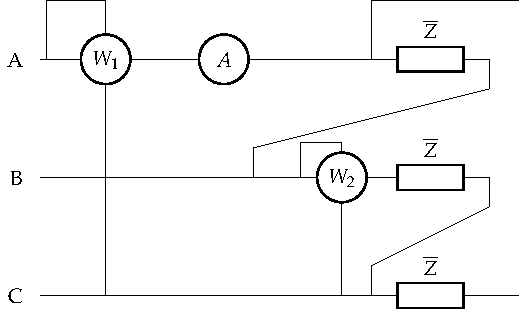
\includegraphics[width=\linewidth]{figuras/dosvat_triangulo.pdf}
\end{minipage}


\subsection*{Solución}

Para solucionar las preguntas en este problema, antes de calcular
nada, podemos extraer la siguiente información del enunciado:
\begin{itemize} % para incluir viñetas
\item Se tiene una sola carga trifásica equilibrada de valor $Z$ y con
  $\cos{\phi}=0,6\rightarrow \qty{53.13}{\degree}$ en retraso. Esto
  significa que la impedancia $\overline{Z}$ es de carácter inductivo
  y su potencia reactiva será positiva.
\item Se tiene una secuencia de fases directa ABC. Esto significa que
  el sistema de alimentación tiene las siguientes tensiones de línea:
  $\overline{U}_{AB}={U_{AB}\phase{\ang{120}}}\unit{\volt}$,
  $\overline{U}_{BC}={U_{BC}\phase{\ang{0}}}\unit{\volt}$
  y
  $\overline{U}_{CA}={U_{CA}\phase{\ang{-120}}}\unit{\volt}$. Así
  pues, las tensiones de fase son:
  $\overline{U}_{A}={U_{A}\phase{\ang{90}}}\unit{\volt}$,
  $\overline{U}_{B}={U_{B}\phase{\ang{-30}}}\unit{\volt}$
  y
  $\overline{U}_{C}={U_{C}\phase{\ang{-150}}}\unit{\volt}$.
\item Anotamos la frecuencia de red de valor $\qty{60}{\hertz}$ por si
  hemos de calcular alguna reactancia inductiva y/o capacitiva.
\item La potencia activa total que demanda el triángulo de impedancia
  $\overline{Z}$ es de valor $P_T=\qty{51984}{\watt}$. De este valor,
  sacamos como conclusión que cada impedancia $\overline{Z}$ del
  triángulo consume un tercio de dicha potencia activa al ser un
  receptor equilibrado.
\item El vatímetro $W_2$ está conectado midiendo la intensidad
  $\overline{I}_{BC}$ y la tensión $\overline{U}_{BC}$, es decir, nos
  da el valor de la potencia activa que disipa la fase BC del
  triángulo, cuyo valor ya sabemos que es:
  \[
    W_2=\dfrac{P_T}{3}=\dfrac{51984}{3}=\qty{17328}{\watt}
  \]
\item El amperímetro dispuesto en la línea A mide el valor eficaz de
  $\qty[parse-numbers=false]{76\sqrt{3}}{\ampere}$. Esto significa que,
  al tener un receptor equilibrado conectado en triángulo, las
  intensidades por las otras dos líneas B y C tienen el mismo valor de
  intensidad de valor eficaz de
  $\qty[parse-numbers=false]{76\sqrt{3}}{\ampere}$.
\item También, al ser un receptor equilibrado conectado en triángulo,
  las intensidades $\overline{I}_{AB}$, $\overline{I}_{BC}$ e
  $\overline{I}_{CA}$ que circulan dentro del triángulo, toman por
  valor eficaz:
  \[
    \dfrac{76\sqrt{3}}{\sqrt{3}}=\qty{76}{\ampere}
  \]
\item Los argumentos de las intensidades dentro de triángulo se pueden
  obtener del propio enunciado. Cada intensidad $\overline{I}_{AB}$,
  $\overline{I}_{BC}$ e $\overline{I}_{CA}$ retrasa
  $\ang{53,13}$ a las tensiones $\overline{U}_{AB}$,
  $\overline{U}_{BC}$ y $\overline{U}_{CA}$ correspondientes, es
  decir, la intensidad $\overline{I}_{AB}$ tiene un argumento de valor
  $120-53,13=\ang{66,87}$, la intensidad $\overline{I}_{BC}$
  tiene un argumento de valor $0-53,13=\ang{-53,13}$ y la
  intensidad $\overline{I}_{CA}$ tiene un argumento de valor
  $-120-53,13=\ang{-153,13}$.
\item Los argumentos de las intensidades de línea también se pueden
  obtener del propio enunciado. Cada intensidad $\overline{I}_A$,
  $\overline{I}_B$ e $\overline{I}_C$ retrasa $\ang{53,13}$ a
  las tensiones del sistema de alimentación $\overline{U}_A$,
  $\overline{U}_B$ y $\overline{U}_C$ correspondientes, es decir, la
  intensidad $\overline{I}_A$ tiene un argumento de valor
  $90-53,13=\ang{36,87}$, la intensidad $\overline{I}_B$ tiene
  un argumento de valor $-30-53,13=\ang{-83,13}$ y la
  intensidad $\overline{I}_C$ tiene un argumento de valor
  $-150-53,13=\ang{-203,13}$.
\end{itemize}

Tras estas consideraciones, se pueden iniciar los cálculos necesarios
para responder a las preguntas del problema:
\begin{enumerate}
\item Medida de los vatímetros 1 y 2.
    
  La lectura del vatímetro 1, según está conectado, es la siguiente:
  \[ [W_1]=\Re(\overline{U}_{AC}\cdot \overline{I} _A)=U_{AC}\cdot I_A\cdot
    \cos(\langle \overline{U}_{AC}, \overline{I}_A \rangle)
  \]

  Se desconoce el módulo de la tensión $\overline{U}_{AC}$. Se calcula
  a partir del vatímetro 2 cuya lectura es de
  $[W_2]=\qty{17328}{\watt}$:
  \begin{align*}
 [W_2] &=\Re(\overline{U}_{BC} \cdot \overline{I}_{BC})=U_{BC}\cdot
    I_{BC}\cdot \cos(\langle \overline{U_{BC}},
         \overline{I_{BC}}\rangle)\\
    17328&=U_{BC}\cdot 76\cdot
    0.6\Rightarrow U_{BC}=\qty{380}{\volt}
  \end{align*}
  Por tanto, al ser un sistema equilibrado ($U_{AB}=U_{BC}=U_{CA}$), y
  sabiendo que
  $\overline{U}_{AC}=-\overline{U}_{CA}=U_{CA}\phase{-120+180}=\qty[parse-numbers=false]{380\phase{\ang{60}}}{\volt}$,
  la lectura del vatímetro 1:
  \[ [W_1]=\Re(\overline{U}_{AC}\cdot \overline{I}_A)=U_{AC}\cdot I_A\cdot
    \cos(\langle \overline{U}_{AC}, \overline{I}_A \rangle)=380\cdot
    76\sqrt{3}\cdot \cos(\langle60;36.87\rangle)=\qty{46001}{\watt}
  \]

\item Valor de la impedancia $\overline{Z}$ en forma módulo-argumento.

  Al conocer ya el valor de la tensión a la que está alimentada y la
  intensidad que circula por ella, se obtiene su valor fácilmente a
  partir de la ley de Ohm:
  \[
    \overline{Z}=\dfrac{\overline{U}_{AB}}{\overline{I}_{AB}}=\dfrac{380\phase{120}}{76\phase{66.87}}={5\phase{\ang{53.13}}}\unit{\ohm}
  \]

\item Valor de la capacidad mínima para mejorar el factor de potencia
  a $0.95$ en retraso.




\item Valor de la impedancia equivalente en estrella.


\end{enumerate}

\section{Enunciado}
Un sistema trifásico a cuatro hilos de $\qty{200}{\volt}$ a $\qty{50}{\hertz}$ y secuencia de fases directa está constituido por un motor a cuatro hilos de $\qty{3200}{\watt}$ de potencia y factor de potencia de 0.9, y un triángulo de impedancia $20\phase{\ang{30}}\unit{\ohm}$. Con esta información se debe determinar:

\begin{enumerate}
\item Impedancia equivalente del motor.
\item Impedancia equivalente de todo el sistema.
\end{enumerate}

\subsection*{Solución}

\begin{enumerate}
\item Para calcular la impedancia del motor necesitamos obtener la corriente que lo alimenta. Dado que tenemos la potencia activa y su factor de potencia el cálculo es inmediato:

  \[
    P_m = \sqrt{3} \cdot U \cdot I_m \cdot \cos(\theta_m) \rightarrow I_m = \qty{10.26}{\ampere}.
  \]
Además, el ángulo se obtiene del factor de potencia: $\theta_m = \arccos(0.9) = \ang{25.84}$.
  Con estos valores podemos calcular la impedancia equivalente en triángulo:

  \[
    \overline{Z}_{m\triangle} = \frac{U}{I_{mf}}\phase{\theta_m} = \frac{200}{10.26/\sqrt{3}}\phase{\ang{25.84}} = 33.76\phase{\ang{25.84}}\unit{\ohm}
  \]

  Y en estrella:

\[
  \overline{Z}_{mY} = \frac{U_f}{I_{m}}\phase{\theta_m} = \frac{200/\sqrt{3}}{10.26}\phase{\ang{25.84}} = 11.25\phase{\ang{25.84}}\unit{\ohm}
  \]
 
\item Para calcular la impedancia equivalente del conjunto necesitamos obtener la corriente total del sistema y, por tanto, el triángulo de potencias total. En primer lugar, el motor:

  \begin{align*}
    P_m &= \qty{3200}{\watt}\\
    Q_m &= P_m \tan(25.84) = \qty{1549.83}{\VAr}
  \end{align*}

  A continuación, la impedancia. Primer debemos obtener la corriente de esta impedancia:

  \begin{align*}
    I_{zf} &= \frac{U}{Z_\triangle} = \qty{10}{\ampere}\\
    I_z &= \sqrt{3}\cdot I_{zf} = 10\sqrt{3}\unit{\ampere}
  \end{align*}
  Y ya podemos obtener las potencias de esta impedancia:
  \begin{align*}
    P_z &= \sqrt{3}\cdot U \cdot I_z \cdot \cos(\ang{30}) = \qty{5196.2}{\watt}\\
    Q_z &= P_m \tan(30) = \qty{3000}{\VAr}
  \end{align*}

  Aplicando Boucherot:

  \begin{align*}
    P &= P_m + P_z = \qty{8396.2}{\watt}\\
    Q &= Q_m + Q_z = \qty{4549.8}{\VAr}\\
    S & = \sqrt{P^2 + Q^2} = \qty{9549.7}{\voltampere}
  \end{align*}

  Con estos resultados obtenemos la corriente total y el ángulo de la impedancia equivalente:

  \begin{align*}
    I &= \frac{S}{\sqrt{3} U} = \qty{27.6}{\ampere}\\
    \theta &= \arctan(\frac{Q}{P}) = \ang{28.45}
  \end{align*}

  Por tanto,

  \begin{align*}
    \overline{Z}_{\triangle} &= \frac{U}{I_{f}}\phase{\theta} = 12.57\phase{\ang{28.45}}\unit{\ohm}\\
    \overline{Z}_{Y} &= \frac{U_f}{I}\phase{\theta} = 4.19\phase{\ang{28.45}}\unit{\ohm}
  \end{align*}
\end{enumerate}

\section{Enunciado}

En el circuito de la figura la tensión es $275\sqrt{3}\unit{\volt}$. Los motores 1 y 2 tienen factores de potencia 0.96 y 0.8, respectivamente. El vatímetro $W_a$ da una lectura de $2420\sqrt{3}\unit{\watt}$. Al medir las intensidades de los motores se comprueba que son iguales en ambos. Con esta información se debe determinar:

\begin{enumerate}
\item Secuencia de fases del sistema.
\item Lectura del vatímetro $W_b$.
\item Impedancias de cada uno de los motores e impedancia equivalente del conjunto.
\end{enumerate}

\begin{center}
  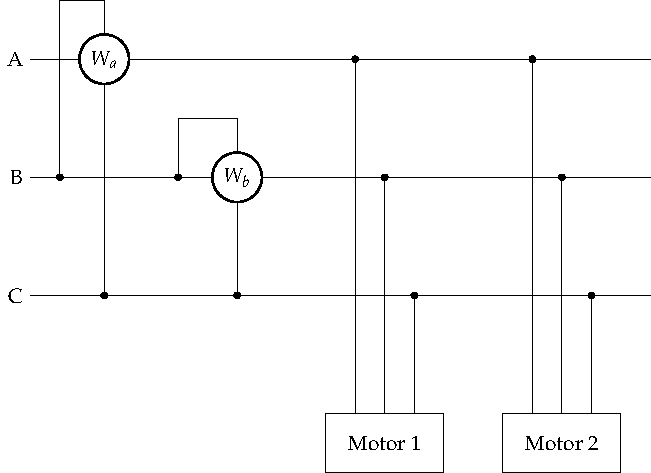
\includegraphics{figuras/BT3_13}
\end{center}

\subsection*{Solución}

\begin{enumerate}
\item El sistema está equilibrado y es inductivo. Por tanto, la reactiva total es positiva. Por otra parte:

  \[
    W_a = \pm \frac{Q}{\sqrt{3}}
  \]

  Dado que la lectura del vatímetro es positiva y la potencia reactiva total también es positiva, hay que elegir el signo positivo. Este vatímetro está conectado entre B y C, luego se trata de una SFD.
\item Con la lectura del vatímetro $W_a$ tenemos la potencia reactiva total del sistema. Por Boucherot sería:

  \[
    Q = Q_1 + Q_2 = \sqrt{3} \cdot U \cdot I_1 (\sen(\theta_1) + \sen(\theta_2))
  \]
  donde se ha tenido en cuenta que las corrientes de los dos motores son iguales, $I_1 = I_2$. De esta expresión podemos obtener el valor de estas corrientes.

  \[
    I_1 = I_2 = \frac{Q}{\sqrt{3} \cdot U \cdot (\sen(\theta_1) + \sen(\theta_2))} = \qty{10}{\ampere}
  \]

  Con una operación similar para la potencia activa:

  \[
    P = P_1 + P_2 = \sqrt{3} \cdot U \cdot I_1 (\cos(\theta_1) + \cos(\theta_2)) = \qty{14520}{\watt}
  \]

  Con este resultado podemos calcular la lectura del vatímetro $W_b$. Este vatímetro forma parte de un montaje Aron. Si añadimos un vatímetro ficticio en la fase A, $W_x$ , tendríamos:

  \begin{align*}
    W_x + W_b &= P\\
    W_x - W_b &= Q/\sqrt{3} = W_a
  \end{align*}

  Por tanto:

  \[
    W_b = 1/2 \cdot (P - W_a) = \qty{5164.2}{\watt}
  \]
  
\item Las impedancias de los dos motores podemos calcularlas con la tensión del sistema y las corrientes que los alimentan, calculadas en el apartado anterior, $I_1 = I_2 = \qty{10}{\ampere}$.

    \begin{align*}
      \overline{Z}_{1Y} &= \frac{U_f}{I_1}\phase{\theta_1} = 27.5\phase{\ang{16.26}}\unit{\ohm}\\
      \overline{Z}_{2Y} &= \frac{U_f}{I_2}\phase{\theta_2} = 27.5\phase{\ang{36.87}}\unit{\ohm}
  \end{align*}

  Para calcular la impedancia equivalente del conjunto necesitamos la corriente total y el ángulo, que se obtienen del triángulo de potencias:

  \begin{align*}
    S &= \sqrt{P^2 + Q^2} = \qty{16233.9}{\voltampere}\\
    I &= \frac{S}{\sqrt{3} \cdot U} = \qty{19.7}{\ampere}\\
    \theta &= \arctan{\frac{Q}{P}} = \ang{26.56}
  \end{align*}
  Por tanto:

  \[
    \overline{Z}_{Y} = \frac{U_f}{I}\phase{\theta} = 13.97\phase{\ang{26.56}}\unit{\ohm}
  \]

  A este mismo resultado se puede llegar calculando la impedancia equivalente del paralelo de $\overline{Z}_{1Y}$ y $\overline{Z}_{2Y}$:

  \[
    \overline{Z}_Y = \frac{\overline{Z}_{1Y} \cdot \overline{Z}_{2Y}}{\overline{Z}_{1Y} + \overline{Z}_{2Y}} = 13.97\phase{\ang{26.56}}\unit{\ohm}
  \]
\end{enumerate}

%%% Local Variables:
%%% mode: latex
%%% TeX-master: "Problemas_TC"
%%% ispell-local-dictionary: "castellano"
%%% End:
